\item \points{25} {\bf Linear Classifiers (GDA)}

In PSET 1, you covered logistic regression in problem 3. In this problem, we apply a generative linear classifier, Gaussian discriminant
analysis (GDA), on the same datasets. Both of the algorithms find a linear decision boundary that
separates the data into two classes, but make different assumptions. Our goal
in this problem is to get a deeper understanding of the similarities and
differences (and, strengths and weaknesses) of these two algorithms.

For this problem, we will consider the same two datasets, along with starter codes provided in the following
files:
\begin{center}
\begin{itemize} %[label=\roman*.]
	\item \url{src/linearclass/ds1_{train,valid}.csv}
	\item \url{src/linearclass/ds2_{train,valid}.csv}
        \item \url{src/linearclass/gda.py}
\end{itemize}
\end{center}
Recall that each file contains $\nexp$ examples, one example $(x^{(i)}, y^{(i)})$ per row.
In particular, the $i$-th row contains columns $x^{(i)}_1\in\Re$,
$x^{(i)}_2\in\Re$, and $y^{(i)}\in\{0, 1\}$.

\begin{enumerate}

	\item \subquestionpoints{5}
In GDA we model the joint distribution of $(x, y)$ by the following
equations:
%
\begin{eqnarray*}
	p(y) &=& \begin{cases}
	\phi & \mbox{if~} y = 1 \\
	1 - \phi & \mbox{if~} y = 0 \end{cases} \\
	p(x | y=0) &=& \frac{1}{(2\pi)^{\di/2} |\Sigma|^{1/2}}
		\exp\left(-\frac{1}{2}(x-\mu_{0})^T \Sigma^{-1} (x-\mu_{0})\right) \\
	p(x | y=1) &=& \frac{1}{(2\pi)^{\di/2} |\Sigma|^{1/2}}
		\exp\left(-\frac{1}{2}(x-\mu_1)^T \Sigma^{-1} (x-\mu_1) \right),
\end{eqnarray*}
%
where $\phi$, $\mu_0$, $\mu_1$, and $\Sigma$ are the parameters of our model.

Suppose we have already fit $\phi$, $\mu_0$, $\mu_1$, and $\Sigma$, and now
want to predict $y$ given a new point $x$. To show that GDA results in a
classifier that has a linear decision boundary, show the posterior distribution
can be written as
%
\begin{equation*}
	p(y = 1\mid x; \phi, \mu_0, \mu_1, \Sigma)
	= \frac{1}{1 + \exp(-(\theta^T x + \theta_0))},
\end{equation*}
%
where $\theta\in\Re^\di$ and $\theta_{0}\in\Re$ are appropriate functions of
$\phi$, $\Sigma$, $\mu_0$, and $\mu_1$. State the value of $\theta$ and $\theta_0$ as a function of $\phi, \mu_0, \mu_1, \Sigma$ explicitly.


        \ifnum\solutions=1 {
            \begin{answer}

$$
p(y=1\mid x;\phi,\mu_0,\mu_1,\Sigma)
= \frac{p(x\mid y=1)p(y=1)}
       {p(x\mid y=1)p(y=1) + p(x\mid y=0)p(y=0)}
$$
Rewrite the posterior following $\frac{a}{a+b} = \frac{1}{a^{-1}} \frac{1}{a+b} = \frac{1}{1+a^{-1}b}$
$$
p(y=1\mid x;\phi,\mu_0,\mu_1,\Sigma)
= \frac{1}
       {1 + \frac{p(x\mid y=0)p(y=0)}{p(x\mid y=1)p(y=1)}}
$$
Then, to comply with the logistics form:
$$
p(y=1\mid x;\phi,\mu_0,\mu_1,\Sigma)
= \frac{1}
       {1 + \exp \log \left( \frac{p(x\mid y=0)p(y=0)}{p(x\mid y=1)p(y=1)} \right)}
$$
$$
\log\frac{p(x\mid y=0)p(y=0)}{p(x\mid y=1)p(y=1)}
= \log \frac{p(x\mid y=0)}{p(x\mid y=1)}
+ \log \frac{p(y=0)}{p(y=1)}
$$
And
$$
p(x\mid y=i)
= \frac{1}{(2\pi)^{d/2}|\Sigma|^{1/2}}
  \exp\!\left(-\frac12(x-\mu_i)^{\top}\Sigma^{-1}(x-\mu_i)\right),
  \quad i\in\{0,1\}.
$$
So
$$
\begin{align}
\log \frac{p(x\mid y=0)}{p(x\mid y=1)}
&= -\frac{1}{2}\Big[
(x-\mu_0)^{\top}\Sigma^{-1}(x-\mu_0)
- (x-\mu_1)^{\top}\Sigma^{-1}(x-\mu_1)
\Big] \\
&= x^{\top}\Sigma^{-1}(\mu_0-\mu_1)
   + \tfrac{1}{2}(\mu_1^{\top}\Sigma^{-1}\mu_1 - \mu_0^{\top}\Sigma^{-1}\mu_0)
\end{align}
$$
$$
\log \frac{p(y=0)}{p(y=1)} = \log \frac{1-\phi}{\phi} = - \log \frac{\phi}{1-\phi}
$$
$$
\exp \log \left( \frac{p(x\mid y=0)p(y=0)}{p(x\mid y=1)p(y=1)} \right)
= \exp \left(
(\mu_0-\mu_1)^{\top}\Sigma^{-1}x
   + \tfrac{1}{2}(\mu_1^{\top}\Sigma^{-1}\mu_1 - \mu_0^{\top}\Sigma^{-1}\mu_0)
+ \log \frac{1-\phi}{\phi}
\right)
$$
Then, the values of $\theta$ and $\theta_{0}$ to match the logistic form are:

$$
\boxed{
\theta = \Sigma^{-1}(\mu_{1}-\mu_{0})
}
$$
$$
\boxed{
\theta_{0} 
= \tfrac{1}{2}(\mu_0^{\top}\Sigma^{-1}\mu_0 - \mu_1^{\top}\Sigma^{-1}\mu_1)
+ \log \frac{\phi}{1-\phi}
}
$$
\end{answer}

        }\fi

	\item \subquestionpoints{7} Given the dataset, we claim that the maximum
  likelihood estimates of the parameters are given by
  \begin{eqnarray*}
    \phi &=& \frac{1}{\nexp} \sum_{i=1}^\nexp 1\{y^{(i)} = 1\} \\
\mu_{0} &=& \frac{\sum_{i=1}^\nexp 1\{y^{(i)} = {0}\} x^{(i)}}{\sum_{i=1}^\nexp
1\{y^{(i)} = {0}\}} \\
\mu_1 &=& \frac{\sum_{i=1}^\nexp 1\{y^{(i)} = 1\} x^{(i)}}{\sum_{i=1}^\nexp 1\{y^{(i)}
= 1\}} \\
\Sigma &=& \frac{1}{\nexp} \sum_{i=1}^\nexp (x^{(i)} - \mu_{y^{(i)}}) (x^{(i)} -
\mu_{y^{(i)}})^T
  \end{eqnarray*}
  The log-likelihood of the data is
  \begin{eqnarray*}
\ell(\phi, \mu_{0}, \mu_1, \Sigma) &=& \log \prod_{i=1}^\nexp p(x^{(i)} , y^{(i)};
\phi, \mu_{0}, \mu_1, \Sigma) \\
&=& \log \prod_{i=1}^\nexp p(x^{(i)} | y^{(i)}; \mu_{0}, \mu_1, \Sigma) p(y^{(i)};
\phi).
  \end{eqnarray*}
By maximizing $\ell$ with respect to the four parameters,
prove that the maximum likelihood estimates of $\phi$, $\mu_{0}, \mu_1$, and
$\Sigma$ are indeed as given in the formulas above.  (You may assume that there
is at least one positive and one negative example, so that the denominators in
the definitions of $\mu_{0}$ and $\mu_1$ above are non-zero.)


        \ifnum\solutions=1 {
            \begin{answer}
   

\end{answer}

        } \fi

	\item \subquestionpoints{10} \textbf{Coding problem.}
In \texttt{src/linearclass/gda.py}, fill in the code to
calculate $\phi$, $\mu_{0}$, $\mu_{1}$, and $\Sigma$, use these parameters
to derive $\theta$, and use the resulting GDA model to make predictions on the
validation set. Make sure to write your model's predictions on
the validation set to the file specified in the code.

Include two plots of the \textbf{validation data} for both datasets with $x_1$ on the horizontal axis and $x_2$ on the vertical axis.
To visualize the two classes, use a different symbol for examples $x^{(i)}$
with $y^{(i)} = 0$ than for those with $y^{(i)} = 1$. On the same figures, plot the decision boundary
found by GDA (i.e, line corresponding to $p(y|x) = 0.5$).

Note that your code should be run inside the \texttt{src/linearclass/} directory.


        \ifnum\solutions=1 {
            \begin{answer}
Figures \ref{fig:GDA_pred_1} and \ref{fig:GDA_pred_2} show classifier predictions for both datasets

\begin{figure}
    \centering
    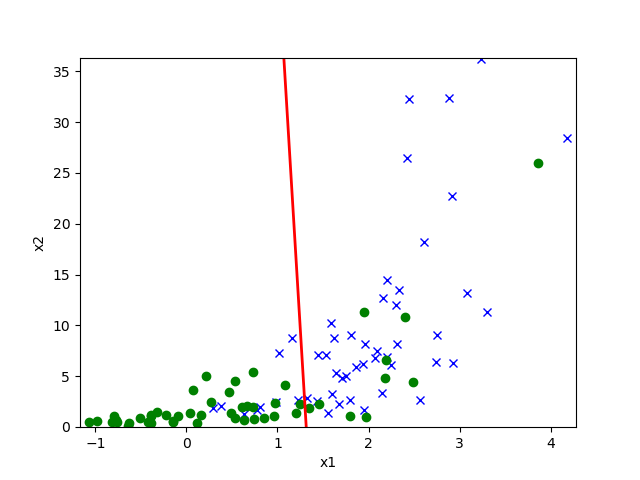
\includegraphics[width=0.8\linewidth]{/home/saveasmtz/Documents/CS229/ps2/tex/imgs/gda_pred_1.png}
    \caption{GDA on Dataset 1}
    \label{fig:GDA_pred_1}
\end{figure}

\begin{figure}
    \centering
    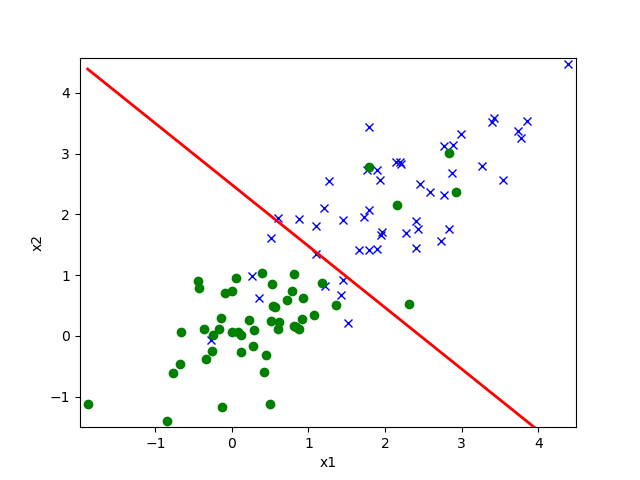
\includegraphics[width=0.8\linewidth]{/home/saveasmtz/Documents/CS229/ps2/tex/imgs/gda_pred_2.png}
    \caption{GDA on Dataset 2}
    \label{fig:GDA_pred_2}
\end{figure}


\end{answer}

        } \fi

	\item \subquestionpoints{2}
For both datasets, compare the validation set plots obtained in part (c) and PSET 1, Problem 3, part (b)
from GDA and logistic regression respectively, and briefly comment on your observation
in a couple of lines.
On which dataset does GDA seem to perform worse than logistic regression? Why might this be the case?


        \ifnum\solutions=1 {
            \begin{answer}
Dataset 1, maybe because the covariance matrices for each classifier are not really the same.
\end{answer}

        } \fi

	\item \subquestionpoints{1} For the dataset where GDA performed worse in
part (d), can you find a transformation of the $x^{(i)}$'s such
that GDA performs significantly better? What might this transformation be?


        \ifnum\solutions=1{
            \begin{answer}

\end{answer}

        }\fi

\end{enumerate}
